\documentclass[12pt,a4paper]{article}

\usepackage[utf8]{inputenc}
\usepackage[T1]{fontenc}
\usepackage[polish]{babel}
\usepackage{lmodern}
\usepackage{geometry}
\usepackage{graphicx}
\usepackage{xcolor}
\usepackage{booktabs}
\usepackage{tabularx}
\usepackage{longtable}
\usepackage{array}
\usepackage{enumitem}
\usepackage{float}
\usepackage{listings}
\usepackage{fancyhdr}
\usepackage{hyperref}
\usepackage{url}

\geometry{left=2.5cm,right=2.5cm,top=2.8cm,bottom=2.7cm}
\setlength{\headheight}{28pt}
\setlength{\parskip}{0.35em}
\setlength{\parindent}{0pt}
\renewcommand{\arraystretch}{1.2}
\emergencystretch=2em

\definecolor{navy}{RGB}{18,37,50}
\definecolor{orange}{RGB}{226,113,36}
\definecolor{lightgray}{RGB}{245,247,249}
\definecolor{codeblue}{RGB}{32,75,130}
\definecolor{codegreen}{RGB}{35,115,75}

\hypersetup{
    colorlinks=true,
    linkcolor=navy,
    urlcolor=codeblue,
    citecolor=navy,
    pdftitle={Dokumentacja projektu AutoPart Store},
    pdfauthor={Jan Wójcik, Kacper Tworek}
}

\pagestyle{fancy}
\fancyhf{}
\fancyhead[L]{\nouppercase{\leftmark}}
\fancyhead[R]{AutoPart Store}
\fancyfoot[C]{\footnotesize Inżynieria Oprogramowania A* \quad | \quad \thepage}
\renewcommand{\headrulewidth}{0.4pt}
\renewcommand{\footrulewidth}{0.4pt}

\lstdefinelanguage{CSharp}{
    morekeywords={using,namespace,public,private,protected,internal,class,static,readonly,
        async,await,return,if,else,new,var,void,string,int,decimal,bool,Task,ActionResult,
        IActionResult,Include,Where,Select,OrderBy,AddScoped,AddDbContext,GetRequiredService},
    sensitive=true,
    morecomment=[l]{//},
    morestring=[b]"
}
\lstset{
    language=CSharp,
    basicstyle=\ttfamily\footnotesize,
    keywordstyle=\color{codeblue}\bfseries,
    commentstyle=\color{codegreen},
    stringstyle=\color{orange},
    backgroundcolor=\color{lightgray},
    frame=single,
    rulecolor=\color{black!20},
    numbers=left,
    numberstyle=\tiny\color{black!55},
    numbersep=8pt,
    breaklines=true,
    columns=fullflexible,
    keepspaces=true,
    showstringspaces=false,
    literate=
        {ą}{{\k{a}}}1 {ć}{{\'c}}1 {ę}{{\k{e}}}1 {ł}{{\l{}}}1
        {ń}{{\'n}}1 {ó}{{\'o}}1 {ś}{{\'s}}1 {ź}{{\'z}}1 {ż}{{\.z}}1
        {Ą}{{\k{A}}}1 {Ć}{{\'C}}1 {Ę}{{\k{E}}}1 {Ł}{{\L{}}}1
        {Ń}{{\'N}}1 {Ó}{{\'O}}1 {Ś}{{\'S}}1 {Ź}{{\'Z}}1 {Ż}{{\.Z}}1
}

\begin{document}

\begin{titlepage}
    \thispagestyle{empty}
    \centering
    \vspace*{1cm}
    {\Large\scshape Akademia Nauk Stosowanych w Nowym Sączu\par}
    \vspace{0.25cm}
    {\large\scshape Wydział Nauk Inżynieryjnych\par}
    \vspace{0.8cm}
    \rule{\textwidth}{1.2pt}\par
    \vspace{1.8cm}
    {\Large Inżynieria Oprogramowania A*\par}
    \vspace{0.8cm}
    {\huge\bfseries\color{navy} Dokumentacja projektu\par}
    \vspace{0.35cm}
    {\LARGE\bfseries\color{orange} AutoPart Store\par}
    \vspace{0.7cm}
    {\large Internetowy sklep z częściami i akcesoriami samochodowymi\par}
    \vspace{1cm}
    \rule{0.55\textwidth}{0.5pt}\par
    \vfill
    \begin{minipage}{0.45\textwidth}
        \raggedright
        \textbf{Prowadzący:}\\
        mgr inż. Józef Wójcik
    \end{minipage}
    \begin{minipage}{0.45\textwidth}
        \raggedleft
        \textbf{Autorzy:}\\
        Jan Wójcik\\
        Kacper Tworek\\
        Grupa P2
    \end{minipage}
    \vfill
    {\large Nowy Sącz, 24 listopada 2026\par}
\end{titlepage}

\pagenumbering{roman}
\tableofcontents
\newpage
\pagenumbering{arabic}

\section*{Streszczenie}
\addcontentsline{toc}{section}{Streszczenie}
Dokument opisuje projekt i aktualny stan aplikacji internetowej AutoPart Store:
jej wymagania, architekturę, model danych, najważniejsze procesy, kolejne sprinty,
zabezpieczenia, testy oraz możliwości wdrożenia. Opracowanie powstało na podstawie
dostarczonego szkicu dokumentacji, kodu źródłowego projektu, checklisty UAT oraz
zrzutu ekranu panelu raportów sprzedaży.

W opisie rozróżniono funkcje rzeczywiście zaimplementowane od założeń, które nie
znajdują potwierdzenia w kodzie lub wymagają dodatkowych prac. W szczególności
aplikacja nie zawiera katalogu dopasowania części do pojazdu według VIN/OEM,
nie prowadzi osobnego dziennika transakcji magazynowych, a symulator płatności
jest ograniczony do środowiska deweloperskiego. Obecna wersja jest aplikacją
ASP.NET Core MVC z bazą SQLite; nie jest statyczną stroną możliwą do uruchomienia
na Netlify jako kompletny system.

\textbf{Słowa kluczowe:} ASP.NET Core MVC, sklep internetowy, SQLite, EF Core,
zamówienia, raport sprzedaży, UAT.

\section{Wprowadzenie}

\subsection{Cel dokumentu}
Celem dokumentu jest przedstawienie systemu AutoPart Store w sposób umożliwiający
zrozumienie jego przeznaczenia, struktury i sposobu działania. Dokument może
stanowić materiał projektowy i prezentacyjny, a także punkt wyjścia do dalszego
rozwoju aplikacji. Opis funkcjonalności odnosi się do wersji kodu dostępnej
w repozytorium w dniu 24 listopada 2026 r.

\subsection{Cel i zakres systemu}
AutoPart Store jest aplikacją webową wspierającą podstawową sprzedaż części
i akcesoriów samochodowych. Klient może przeglądać katalog, filtrować produkty,
zarządzać koszykiem, złożyć zamówienie w środowisku testowym oraz przeglądać
własną historię zakupów. Pracownik obsługuje kartotekę produktów i zamówienia,
a administrator zarządza kontami, rolami i raportami sprzedaży.

System obejmuje:
\begin{itemize}[leftmargin=*]
    \item rejestrację, logowanie i autoryzację opartą na rolach;
    \item katalog produktów z kategoriami i podkategoriami;
    \item wyszukiwanie tekstowe oraz filtrowanie po kategorii, cenie i dostępności;
    \item koszyk przechowywany w sesji przeglądarki;
    \item składanie zamówień i aktualizację stanów magazynowych;
    \item panel klienta z historią zamówień i pobieraniem dokumentu PDF;
    \item panel obsługi produktów i zamówień;
    \item powiadomienia e-mail konfigurowane przez SMTP;
    \item raport dziennej sprzedaży dostępny dla administratora.
\end{itemize}

\subsection{Granice i ograniczenia}
Aktualny katalog nie przechowuje numerów OEM, VIN, marki/modelu pojazdu ani
reguł dopasowania części do konkretnego samochodu. Wyszukiwanie dotyczy nazwy
i opisu produktu, a nie kompatybilności pojazdu. Aplikacja nie integruje się
z rzeczywistym operatorem płatności, kurierem ani systemem księgowym.

Dokument PDF jest generowany na potrzeby demonstracji procesu. Zawiera
przykładowe dane sprzedawcy, w tym pole NIP wymagające uzupełnienia. Przed
użyciem dokumentu w rzeczywistej sprzedaży należy zweryfikować jego zgodność
z wymaganiami księgowymi oraz uzupełnić dane firmy.

\section{Wymagania}

\subsection{Aktorzy i role}
\begin{table}[H]
\centering
\small
\begin{tabularx}{\textwidth}{@{}l X@{}}
\toprule
\textbf{Rola} & \textbf{Zakres uprawnień}\\
\midrule
Klient & Przeglądanie katalogu, obsługa koszyka, składanie zamówień,
podgląd własnych zamówień i pobieranie własnych faktur PDF.\\
Pracownik & Podgląd i edycja produktów oraz kategorii, przegląd zamówień
i zmiana statusu ich realizacji.\\
Administrator & Uprawnienia pracownika oraz zarządzanie rolami użytkowników
i dostęp do raportów sprzedaży.\\
\bottomrule
\end{tabularx}
\caption{Role i podstawowe uprawnienia w systemie}
\end{table}

\subsection{Wymagania funkcjonalne i stan realizacji}
\begin{longtable}{@{}p{0.11\textwidth}p{0.59\textwidth}p{0.22\textwidth}@{}}
\toprule
\textbf{ID} & \textbf{Wymaganie} & \textbf{Stan}\\
\midrule
\endhead
F-01 & Rejestracja i logowanie klientów oraz obsługa ról. & Zrealizowane\\
F-02 & Zarządzanie produktami: nazwa, opis, kategoria, cena, stan i aktywność. & Zrealizowane\\
F-03 & Zarządzanie kategoriami i podkategoriami. & Zrealizowane\\
F-04 & Wyszukiwanie tekstowe i filtrowanie po kategorii, zakresie cen i dostępności. & Zrealizowane\\
F-05 & Koszyk z dodawaniem, zmianą ilości, usuwaniem pozycji i podsumowaniem. & Zrealizowane\\
F-06 & Składanie zamówień z kontrolą dostępności i zmianą stanów magazynowych. & Zrealizowane\\
F-07 & Panel klienta z listą własnych zamówień i pobieraniem PDF. & Zrealizowane\\
F-08 & Panel personelu do podglądu zamówień i zmiany ich statusu. & Zrealizowane\\
F-09 & Powiadomienia o statusie zamówienia wysyłane przez skonfigurowany SMTP. & Zrealizowane warunkowo\\
F-10 & Generowanie faktury PDF z polskimi znakami i zestawieniem pozycji. & Zrealizowane jako dokument demonstracyjny\\
F-11 & Wirtualny proces płatności. & Dostępny tylko w Development\\
F-12 & Raport sprzedaży za wybrany okres wraz z podsumowaniami i wykresem. & Zrealizowane\\
F-13 & Dopasowanie części do pojazdu według VIN/OEM. & Niezrealizowane\\
F-14 & Osobny, audytowalny rejestr operacji magazynowych. & Niezrealizowane\\
\bottomrule
\end{longtable}

\subsection{Wymagania niefunkcjonalne}
\begin{itemize}[leftmargin=*]
    \item \textbf{Użyteczność:} interfejs MVC w języku polskim, z responsywnymi
    widokami przeznaczonymi do przeglądarek desktopowych i mobilnych.
    \item \textbf{Bezpieczeństwo:} hasła przechowywane jako skróty, uwierzytelnianie
    cookie, autoryzacja ról, walidacja danych, tokeny anty-CSRF dla formularzy
    POST, limit prób logowania i czasowa blokada konta.
    \item \textbf{Integralność danych:} migracje EF Core i transakcyjne operacje
    zakupu oraz przywracania stanów przy anulowaniu zamówienia.
    \item \textbf{Konfigurowalność:} dane SMTP i connection string dostarczane
    z konfiguracji środowiska; sekretów nie należy umieszczać w repozytorium.
    \item \textbf{Utrzymywalność:} rozdzielenie odpowiedzialności pomiędzy
    kontrolery, modele, serwisy, widoki i warstwę dostępu do danych.
\end{itemize}

\section{Technologie i architektura}

\subsection{Stos technologiczny}
\begin{table}[H]
\centering
\begin{tabularx}{\textwidth}{@{}l X@{}}
\toprule
\textbf{Obszar} & \textbf{Technologia}\\
\midrule
Język i platforma & C\# oraz ASP.NET Core MVC, target .NET 10.\\
Widoki & Razor Views (pliki \texttt{.cshtml}), HTML, CSS i JavaScript.\\
Dostęp do danych & Entity Framework Core i migracje Code First.\\
Baza danych & SQLite w bieżącej konfiguracji projektu.\\
Uwierzytelnianie & Cookie Authentication, claims i autoryzacja ról.\\
PDF & QuestPDF.\\
Poczta & SMTP przez \texttt{System.Net.Mail}.\\
Testy & xUnit, \texttt{Microsoft.AspNetCore.Mvc.Testing} i EF Core SQLite.\\
Publikacja & Dockerfile oraz workflow CI w GitHub Actions.\\
\bottomrule
\end{tabularx}
\caption{Technologie użyte w aktualnej wersji aplikacji}
\end{table}

\subsection{Architektura aplikacji}
Aplikacja wykorzystuje wzorzec Model--View--Controller. Żądanie HTTP jest
obsługiwane przez kontroler, który waliduje dane i koordynuje logikę procesu.
Modele domenowe i modele widoków opisują dane, a widoki Razor generują HTML.
Usługi płatności, powiadomień i faktur są wstrzykiwane przez kontener
Dependency Injection. Warstwa EF Core komunikuje się z bazą SQLite.

\begin{figure}[H]
\centering
\small
\fbox{\begin{minipage}{0.92\textwidth}
\centering
Przeglądarka użytkownika
\(\longleftrightarrow\)
Routing ASP.NET Core
\(\longrightarrow\)
Kontrolery MVC
\(\longleftrightarrow\)
Serwisy aplikacyjne\\[0.6em]
\(\hspace{3em}\) Widoki Razor
\(\longleftarrow\)
Kontrolery MVC
\(\qquad\)
Serwisy i kontrolery
\(\longleftrightarrow\)
ApplicationDbContext / EF Core
\(\longleftrightarrow\)
SQLite
\end{minipage}}
\caption{Uproszczony przepływ żądania w architekturze MVC}
\label{fig:architecture}
\end{figure}

\subsection{Struktura repozytorium}
\begin{table}[H]
\centering
\small
\begin{tabularx}{\textwidth}{@{}l X@{}}
\toprule
\textbf{Katalog / plik} & \textbf{Odpowiedzialność}\\
\midrule
\texttt{Controllers/} & Akcje MVC dla kont, katalogu, koszyka, strony głównej i panelu administratora.\\
\texttt{Models/} & Encje EF Core, role i modele formularzy/widoków.\\
\texttt{Data/} & \texttt{ApplicationDbContext} oraz seeder danych Development.\\
\texttt{Services/} & Płatności, SMTP i generowanie PDF.\\
\texttt{Views/} & Widoki Razor, w tym katalog, checkout, historia zamówień i raport.\\
\texttt{Migrations/} & Historia zmian schematu bazy danych.\\
\texttt{Tests/} & Automatyczne testy UAT i ich infrastruktura.\\
\texttt{Dockerfile} & Wieloetapowe budowanie i uruchomienie aplikacji w kontenerze.\\
\texttt{DEPLOYMENT.md} & Wskazówki wdrożeniowe, trwały wolumen i konfiguracja SMTP.\\
\bottomrule
\end{tabularx}
\caption{Najważniejsze elementy repozytorium}
\end{table}

\section{Model danych}

\subsection{Główne encje}
\begin{table}[H]
\centering
\small
\begin{tabularx}{\textwidth}{@{}l X@{}}
\toprule
\textbf{Encja} & \textbf{Znaczenie i najważniejsze dane}\\
\midrule
\texttt{User} & Konto, e-mail, skrót hasła, imię, nazwisko, rola oraz dane blokady logowania.\\
\texttt{Address} & Adres użytkownika wykorzystywany jako adres dostawy zamówienia.\\
\texttt{Category} & Nazwa i opis kategorii oraz opcjonalne powiązanie z kategorią nadrzędną.\\
\texttt{Product} & Nazwa, opis, cena, liczba sztuk, aktywność i identyfikator kategorii.\\
\texttt{Order} & Klient, data, status realizacji, status płatności, numer faktury i suma.\\
\texttt{OrderItem} & Produkt, ilość i cena jednostkowa zapamiętana w chwili zakupu.\\
\bottomrule
\end{tabularx}
\caption{Podstawowe encje modelu domenowego}
\end{table}

\subsection{Relacje}
Użytkownik może mieć wiele adresów i składać wiele zamówień. Zamówienie zawiera
pozycje \texttt{OrderItem}; pozycja zachowuje cenę jednostkową niezależnie od
późniejszej zmiany ceny w katalogu. Produkt należy do kategorii. Kategoria może
wskazywać kategorię nadrzędną, co umożliwia budowę prostego drzewa kategorii.

\begin{table}[H]
\centering
\small
\begin{tabularx}{\textwidth}{@{}l l X@{}}
\toprule
\textbf{Relacja} & \textbf{Krotność} & \textbf{Opis}\\
\midrule
User--Order & 1:N & Jedno konto może posiadać wiele zamówień.\\
Order--OrderItem & 1:N & Zamówienie składa się z jednej lub większej liczby pozycji.\\
Product--OrderItem & 1:N & Ten sam produkt może występować w pozycjach wielu zamówień.\\
Category--Product & 1:N & Kategoria grupuje przypisane produkty.\\
Category--Category & 1:N & Kategoria nadrzędna może mieć podkategorie.\\
\bottomrule
\end{tabularx}
\caption{Najważniejsze relacje danych}
\end{table}

\subsection{Migracje i inicjalizacja bazy}
Schemat bazy jest aktualizowany przez migracje EF Core podczas uruchamiania
aplikacji. W środowisku Development wykonywany jest dodatkowo seeder, który
uzupełnia dane prezentacyjne. Seeder nie jest uruchamiany w Production.
Przy wdrożeniu należy zapewnić kopię zapasową bazy i trwałe miejsce na plik
SQLite, ponieważ efemeryczny system plików hostingu może utracić dane po
restartowaniu kontenera.

\section{Opis procesów}

\subsection{Rejestracja i logowanie}
Formularz rejestracji tworzy konto klienta po sprawdzeniu poprawności danych
i unikalności adresu e-mail. Hasło jest przetwarzane przez
\texttt{PasswordHasher<User>} i w bazie przechowywany jest jego skrót.
Podczas logowania system weryfikuje skrót, tworzy uwierzytelniające cookie
i zapisuje w nim identyfikator, nazwę, e-mail oraz rolę użytkownika.

Nieudane próby są liczone dla konta. Po pięciu nieudanych próbach konto jest
blokowane na 15 minut; dodatkowo żądania logowania z jednego adresu IP są
ograniczane do 10 w ciągu 5 minut. Rola w cookie jest ponownie porównywana
z rolą zapisaną w bazie podczas walidacji sesji.

\subsection{Katalog i wyszukiwanie}
Katalog pokazuje aktywne produkty. Użytkownik może wyszukiwać tekst w nazwie
i opisie, wybrać kategorię nadrzędną lub podkategorię, ustawić minimalną
i maksymalną cenę oraz ograniczyć wyniki do produktów dostępnych. Kategorie
podrzędne mogą być pobierane dynamicznie na podstawie kategorii nadrzędnej.

\subsection{Koszyk i złożenie zamówienia}
Koszyk jest przechowywany w sesji. Przed finalizacją system ponownie pobiera
ceny i stany z bazy, sprawdza poprawność adresu i dostępność zamawianych ilości.
Zmniejszenie stanu produktu wykonuje się warunkową aktualizacją, która wymaga
odpowiedniej liczby sztuk w magazynie. Operacje aktualizacji stanów i zapisu
zamówienia są wykonywane w transakcji bazodanowej.

\begin{enumerate}[leftmargin=*]
    \item Klient dodaje aktywne produkty do koszyka.
    \item W checkout wybiera zapisany adres lub podaje nowy.
    \item Aplikacja ponownie weryfikuje produkty, ilości i cenę.
    \item W Development płatność jest sprawdzana przez symulator.
    \item W transakcji zapisywane jest zamówienie z pozycjami i aktualizowany
    jest stan magazynowy.
    \item Klient trafia na stronę potwierdzenia z kwotą.
    \item Po zatwierdzeniu zakupu może zostać wysłana wiadomość e-mail
    z załączoną fakturą PDF, jeśli SMTP jest aktywny.
\end{enumerate}

Przy anulowaniu zamówienia panel obsługi przywraca ilości na stan magazynowy.
Ponowne przywrócenie anulowanego zamówienia jest ograniczone sprawdzeniem
dostępności produktu. W aktualnej wersji nie istnieje osobna encja
rejestrująca każdą operację magazynową; historia zmian nie jest zatem
pełnym dziennikiem audytowym.

\subsection{Obsługa zamówień}
Administrator i pracownik mogą przeglądać listę zamówień oraz szczegóły
zamówienia. Status realizacji wybierany jest z zestawu dopuszczonych statusów.
Zmiana statusu jest zapisywana w bazie; po zatwierdzeniu aplikacja próbuje
wysłać klientowi e-mail z informacją o nowym stanie realizacji.

\subsection{Faktury PDF i powiadomienia}
Faktura PDF zawiera numer dokumentu, dane klienta, pozycje, ilości, wartości
netto i brutto oraz wyliczenie VAT 23\%. Dokument można pobrać z panelu
klienta dla jego własnego zamówienia. Po zakupie faktura może być dołączona
do wiadomości wysyłanej przez SMTP. Błędy SMTP są rejestrowane w logu;
nie cofają już zapisanej transakcji zakupu.

\textbf{Uwaga:} dokument jest demonstracyjny, a pole NIP sprzedawcy w kodzie
ma wartość \texttt{do uzupełnienia}. Nie należy traktować go jako gotowej
podstawy do wystawiania dokumentów księgowych w sprzedaży produkcyjnej.

\subsection{Raport sprzedaży}
Raport jest dostępny wyłącznie dla administratora. Użytkownik wybiera datę
początkową i końcową; zakres może mieć maksymalnie 366 dni. Raport uwzględnia
zamówienia opłacone i nieanulowane, wylicza przychód, liczbę zamówień oraz
średnią wartość zamówienia i prezentuje przychód w ujęciu dziennym.

Na przekazanym zrzucie ekranu przykładowy zakres od 26.10.2026 do 24.11.2026
pokazuje przychód 38\,131{,}31 zł, 144 opłacone zamówienia i średnią wartość
zamówienia 264{,}80 zł. Są to wartości widoczne na obrazie, a nie stałe
wartości wpisane do aplikacji.

\begin{figure}[H]
\centering
\IfFileExists{figures/analiza-sprzedazy.png}{
    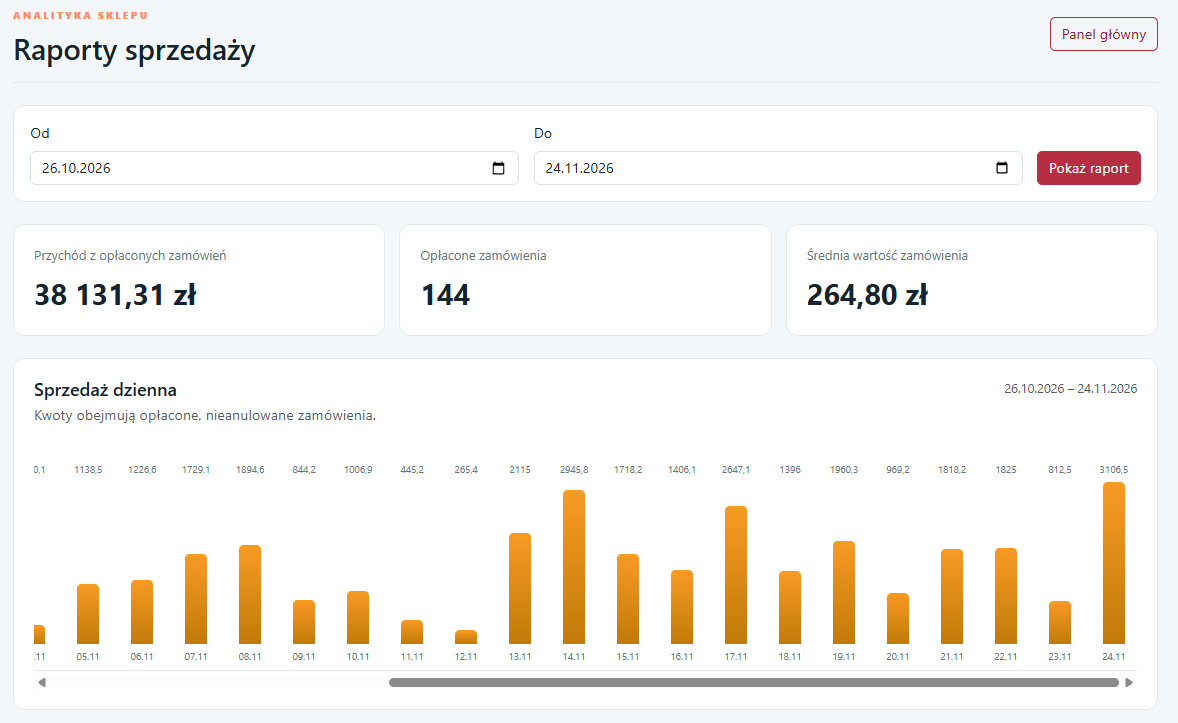
\includegraphics[width=\textwidth]{figures/analiza-sprzedazy.png}
}{
    \fbox{\parbox{0.9\textwidth}{Brak pliku
    \texttt{figures/analiza-sprzedazy.png}. Należy dodać zrzut panelu raportu.}}
}
\caption{Panel raportów sprzedaży przekazany jako materiał do dokumentacji}
\label{fig:sales-report}
\end{figure}

\section{Realizacja prac w sprintach}

\subsection{Sprint 1 -- fundament aplikacji i konta}
\textbf{Cel:} przygotowanie projektu MVC, bazy danych i podstawowych funkcji
kont użytkowników.
\begin{itemize}[leftmargin=*]
    \item utworzenie projektu ASP.NET Core MVC;
    \item konfiguracja SQLite i EF Core;
    \item implementacja rejestracji, logowania i wylogowania;
    \item wprowadzenie ról klienta, pracownika i administratora;
    \item dodanie walidacji formularzy oraz ochrony żądań POST.
\end{itemize}
\textbf{Rezultat:} użytkownicy mogą utworzyć konto, zalogować się i uzyskują
dostęp do funkcji zgodnych ze swoją rolą.

\subsection{Sprint 2 -- katalog i panel administracyjny}
\textbf{Cel:} udostępnienie katalogu produktów, kategoryzacji i operacji
administracyjnych.
\begin{itemize}[leftmargin=*]
    \item modele produktu i kategorii oraz migracje bazy;
    \item kategorie nadrzędne i podkategorie;
    \item wyszukiwanie i filtrowanie katalogu;
    \item dodawanie, edycja i ukrywanie produktów;
    \item zarządzanie kategoriami i zmianą ról użytkowników.
\end{itemize}
\textbf{Rezultat:} katalog jest dostępny publicznie, a zarządzanie asortymentem
jest ograniczone rolami pracownika i administratora.

\subsection{Sprint 3 -- koszyk, zamówienia i stany}
\textbf{Cel:} przeprowadzenie klienta przez proces od koszyka do zapisanego
zamówienia oraz zapewnienie spójności ilości magazynowych.
\begin{itemize}[leftmargin=*]
    \item sesyjny koszyk oraz formularz checkout;
    \item weryfikacja adresu, ceny i dostępności podczas finalizacji;
    \item zapis zamówienia i pozycji w transakcji bazodanowej;
    \item redukcja stanu przy zakupie i jego przywracanie przy anulowaniu;
    \item panel klienta z historią oraz panel personelu do obsługi statusów;
    \item przygotowanie testów i materiałów do wdrożenia kontenerowego.
\end{itemize}
\textbf{Ograniczenie:} w bieżącym kodzie nie ma odrębnego dziennika operacji
magazynowych ani potwierdzenia produkcyjnego wdrożenia. Przygotowano
konfigurację Docker i CI, ale nie jest to równoznaczne z publikacją systemu.

\subsection{Sprint 4 -- płatność demonstracyjna, SMTP i PDF}
\textbf{Cel:} uzupełnienie procesu zakupowego o testową płatność, powiadomienia
oraz dokument PDF.
\begin{itemize}[leftmargin=*]
    \item symulacja zaakceptowanej i odrzuconej płatności w Development;
    \item blokada symulatora poza środowiskiem deweloperskim;
    \item wysyłanie wiadomości SMTP po zakupie i zmianie statusu;
    \item generowanie i pobieranie faktury PDF;
    \item potwierdzenie zamówienia z kwotą i statusem.
\end{itemize}
\textbf{Ograniczenie:} nie skonfigurowano operatora rzeczywistych płatności.
Usługa produkcyjna odrzuca płatności do czasu integracji z operatorem.

\subsection{Sprint 5 -- raportowanie, testy i przygotowanie wdrożenia}
\textbf{Cel:} zapewnienie wglądu w sprzedaż, sprawdzenie kluczowych scenariuszy
oraz przygotowanie aplikacji do demonstracji i dalszego wdrożenia.
\begin{itemize}[leftmargin=*]
    \item raport sprzedaży z filtrem zakresu dat i dziennym wykresem;
    \item ograniczenie raportu do administratora;
    \item testy automatyczne raportów, logowania, płatności i seedera;
    \item checklistę ręcznych testów akceptacyjnych UAT;
    \item poprawki interfejsu responsywnego oraz przygotowanie Dockerfile,
    pipeline CI i instrukcji wdrożenia.
\end{itemize}
\textbf{Ograniczenie:} Netlify nie uruchamia serwera ASP.NET Core MVC.
Wdrożenie całego systemu wymaga hostingu procesu .NET i trwałego magazynu
danych. Na Netlify można publikować wyłącznie niezależny statyczny pokaz
frontendu, bez rzeczywistego logowania i dostępu do bazy.

\section{Bezpieczeństwo i prywatność}

\subsection{Zastosowane mechanizmy}
\begin{itemize}[leftmargin=*]
    \item hasła są haszowane przez wbudowany \texttt{PasswordHasher<User>};
    \item autoryzacja kontrolerów i akcji jest oparta o role;
    \item zmiany danych w formularzach POST korzystają z tokenów anty-CSRF;
    \item logowanie ma limit 10 żądań na 5 minut dla adresu IP oraz blokadę
    konta po pięciu nieudanych próbach na 15 minut;
    \item adres zwrotny po logowaniu jest akceptowany tylko jako lokalny URL;
    \item sesyjne cookie koszyka jest oznaczone jako \texttt{HttpOnly};
    \item aplikacja produkcyjna włącza obsługę błędów i HSTS;
    \item cookie sesji logowania ma ograniczony czas życia, a jej rolę
    waliduje się względem aktualnego rekordu użytkownika;
    \item SMTP i hasła nie powinny być przechowywane w publicznym repozytorium.
\end{itemize}

\subsection{Pozostałe wymagania przed uruchomieniem produkcyjnym}
\begin{enumerate}[leftmargin=*]
    \item Zmienić ujawnione wcześniej dane uwierzytelniające SMTP, jeśli były
    zapisane w pliku lub udostępnione poza zaufanym środowiskiem. Sekrety
    przechowywać w ustawieniach hostingu.
    \item Utworzyć bezpieczny sposób inicjalizacji pierwszego administratora;
    seeder kont prezentacyjnych działa wyłącznie w Development.
    \item Zintegrować rzeczywistego operatora płatności wraz z serwerową
    weryfikacją potwierdzeń i obsługą webhooków.
    \item Uzupełnić prawdziwe dane sprzedawcy i skonsultować format dokumentów
    PDF z osobą odpowiedzialną za księgowość.
    \item Zapewnić kopie zapasowe i trwały dysk dla bazy SQLite albo rozważyć
    produkcyjną bazę zarządzaną.
    \item Wdrożyć HTTPS, monitoring, rotację logów i procedurę odtwarzania
    po awarii.
    \item Przeprowadzić testy obciążeniowe i dodatkowy przegląd bezpieczeństwa
    przed obsługą rzeczywistych klientów.
\end{enumerate}

\section{Testowanie i kryteria akceptacji}

\subsection{Testy automatyczne}
Projekt zawiera testy UAT dotyczące uprawnień i obliczeń raportu, blokowania
konta po nieudanych logowaniach, niedostępności symulatora w Production oraz
idempotencji i zawartości seedera. Ostatnie uruchomienie testów w środowisku
deweloperskim zakończyło się wynikiem 5/5 testów zaliczonych.

\begin{lstlisting}[caption={Polecenie uruchamiające testy UAT w PowerShell}]
dotnet test Tests\AutoPart.Store.UatTests\AutoPart.Store.UatTests.csproj
\end{lstlisting}

\subsection{Scenariusze akceptacyjne}
Poniższe scenariusze pochodzą z checklisty UAT projektu. Należy je wykonywać
w środowisku testowym; samo umieszczenie scenariusza na liście nie oznacza,
że został ręcznie odegrany na wdrożonej instancji.

\begin{longtable}{@{}p{0.12\textwidth}p{0.47\textwidth}p{0.34\textwidth}@{}}
\toprule
\textbf{ID} & \textbf{Scenariusz} & \textbf{Oczekiwany rezultat}\\
\midrule
\endhead
UAT-01 & Klient składa zamówienie z poprawnymi danymi. & Zamówienie zapisuje się, stan maleje, pojawia się potwierdzenie z kwotą.\\
UAT-02 & Klient żąda większej ilości niż dostępna. & Zakup jest blokowany; stan pozostaje bez zmian.\\
UAT-03 & Klient otwiera listę swoich zamówień. & Widzi wyłącznie własne zamówienia i może pobrać PDF.\\
UAT-04 & Personel zmienia status. & Status zostaje zapisany; system próbuje wysłać powiadomienie.\\
UAT-05 & Personel anuluje zamówienie. & Towar z zamówienia wraca na stan magazynowy.\\
UAT-06 & Klient lub pracownik otwiera raport sprzedaży. & Dostęp jest zabroniony; raport jest dostępny administratorowi.\\
UAT-07 & Administrator filtruje raport po datach. & Ujęte są opłacone i nieanulowane zamówienia z zakresu.\\
UAT-08 & Użytkownik pięć razy podaje błędne hasło. & Konto zostaje czasowo zablokowane.\\
UAT-09 & Widoki otwierane są na ekranie 360 px. & Formularze i przyciski pozostają używalne; treść mieści się lub tabele przewijają.\\
UAT-10 & Płatność testowa jest wywołana w Production. & Symulator nie zatwierdza płatności.\\
\bottomrule
\end{longtable}

\section{Wdrożenie i uruchomienie}

\subsection{Uruchomienie lokalne}
Do uruchomienia wymagane jest środowisko .NET 10 SDK. Po pobraniu repozytorium
aplikację można uruchomić poleceniami:

\begin{lstlisting}[caption={Przykładowe polecenia lokalnego uruchomienia}]
dotnet restore
$env:ASPNETCORE_ENVIRONMENT = "Development"
dotnet run --project MyApp.csproj
\end{lstlisting}

W Development aplikacja wykonuje migracje i może uzupełnić bazę danymi
prezentacyjnymi. Hasła i dane dostępu używane do demonstracji nie powinny być
ponownie wykorzystywane w środowisku produkcyjnym.

\subsection{Kontener i hosting}
Repozytorium zawiera wieloetapowy \texttt{Dockerfile}, który publikuje aplikację
i udostępnia port 8080. Konfiguracja obrazu przewiduje bazę SQLite pod ścieżką
\texttt{/app/data/autopartstore.db}; hosting musi zamontować trwały wolumen
w \texttt{/app/data}. Bez niego plik bazy może zostać utracony przy odtworzeniu
konta lub kontenera.

Do działania SMTP należy skonfigurować zmienne środowiskowe:
\begin{table}[H]
\centering
\small
\begin{tabularx}{\textwidth}{@{}l X@{}}
\toprule
\textbf{Zmienna} & \textbf{Znaczenie}\\
\midrule
\texttt{Smtp\_\_Enabled} & Włącza wysyłkę wiadomości.\\
\texttt{Smtp\_\_Host}, \texttt{Smtp\_\_Port} & Serwer i port SMTP.\\
\texttt{Smtp\_\_Username}, \texttt{Smtp\_\_Password} & Dane uwierzytelniające.\\
\texttt{Smtp\_\_EnableSsl} & Konfiguracja szyfrowania połączenia.\\
\texttt{Smtp\_\_From} & Adres nadawcy.\\
\bottomrule
\end{tabularx}
\caption{Konfiguracja poczty w środowisku hostingu}
\end{table}

\subsection{Netlify}
Netlify służy do publikacji statycznych plików, natomiast aplikacja AutoPart
Store wymaga serwera ASP.NET Core, bazy danych, sesji i uwierzytelniania.
W konsekwencji skopiowanie samych plików \texttt{wwwroot} nie udostępni
stron MVC ani logowania. Statyczny pokaz może być osobno przygotowany jako
pliki HTML/CSS/JavaScript, ale nie będzie korzystał z bieżącego backendu.
Pełna aplikacja wymaga hostingu obsługującego kontener .NET lub proces ASP.NET
Core, trwałego miejsca na bazę oraz konfiguracji sekretów.

\section{Wnioski i dalszy rozwój}
W projekcie zaimplementowano główny przepływ sklepu: katalog, konta z rolami,
koszyk, zamówienia, obsługę stanów, historię klienta, powiadomienia, PDF
i raport sprzedaży. Testy automatyczne potwierdzają wybrane reguły raportowania,
ochrony logowania, ograniczenia symulatora i zachowania seedera.

Najważniejsze kolejne kroki to integracja operatora płatności, przygotowanie
produkcyjnego procesu tworzenia administratora, uzupełnienie danych firmy
i formalna walidacja dokumentów, wdrożenie z trwałą bazą i backupem oraz
rozbudowa katalogu o rzeczywiste dopasowanie części do konkretnych pojazdów.
Osobny dziennik zmian stanów magazynowych i testy pełnego checkoutu w
zintegrowanym środowisku również zwiększyłyby możliwość audytu i pewność
wdrożenia.

\section*{Źródła i materiały}
\addcontentsline{toc}{section}{Źródła i materiały}
\begin{enumerate}[leftmargin=*]
    \item Kod źródłowy projektu AutoPart Store, w szczególności
    \texttt{Program.cs}, katalogi \texttt{Controllers/}, \texttt{Models/},
    \texttt{Services/}, \texttt{Data/} i \texttt{Views/}.
    \item \texttt{Tests/UAT-CHECKLIST.md} -- scenariusze akceptacyjne.
    \item Zrzut panelu raportów sprzedaży przekazany do opracowania,
    przedstawiony na rysunku \ref{fig:sales-report}.
    \item Microsoft Learn, dokumentacja ASP.NET Core:
    \url{https://learn.microsoft.com/aspnet/core/}.
    \item Microsoft Learn, dokumentacja Entity Framework Core:
    \url{https://learn.microsoft.com/ef/core/}.
    \item Netlify Docs, dokumentacja publikacji stron statycznych:
    \url{https://docs.netlify.com/}.
\end{enumerate}

\end{document}
